\documentclass{article}

% Symbols
\usepackage{amsfonts}
\usepackage{amsmath}

% Graphics
\usepackage{graphicx}
\usepackage{caption}
%\usepackage{subcaption}
\graphicspath{{../figs/}}

% Tikz
\usepackage{tikz}
\usetikzlibrary{positioning,shapes,arrows,calc,intersections}

% Paths
\newcommand{\figs}{../figs}
\newcommand{\data}{../data}
\newcommand{\code}{../code}

\begin{document}

\section{Model for computer architecture}

\section{Data representation}

\subsection{Memory layout}

Data is stored in binary in the memory:
\begin{itemize}
\item the basic unit is the \textit{byte} consisting of 8 bits,
\item memory may be addressed with a multiple of \textit{bytes},
\item names: \textit{half-word} 16-bit, \textit{word} 32-bit, \textit{double-word} 32-bit, \dots
\end{itemize}

\medskip
Conversion from binary to decimal representation:
\begin{equation*}
\begin{bmatrix}b_k\;b_{k-1}\;\dots\dots b_1\;b_0 \end{bmatrix}_2 = \sum^{k}_{i = 0} b_i\;2^i
\end{equation*}

A bit or binary digit is a value $0$ or $1$.

A sequence of $N$ bits is called a binary word, and $N$ is called the width or size.

The word size can be $8$, $16$, $32$, $64$.

A byte is a sequence of 8 binary digits.

\texttt{char}

\begin{equation*}
\begin{bmatrix}b_7\;b_6\;b_5\;b_4\;b_3\;b_2\;b_1\;b_0 \end{bmatrix}
\end{equation*}

\begin{eqnarray*}
0 :&\qquad\begin{bmatrix}0\;0\;0\;0\;0\;0\;0\;0 \end{bmatrix}\\
1 :&\qquad\begin{bmatrix}0\;0\;0\;0\;0\;0\;0\;1 \end{bmatrix}\\
2 :&\qquad\begin{bmatrix}0\;0\;0\;0\;0\;0\;1\;0 \end{bmatrix}\\
3 :&\qquad\begin{bmatrix}0\;0\;0\;0\;0\;0\;1\;1 \end{bmatrix}\\
4 :&\qquad\begin{bmatrix}0\;0\;0\;0\;0\;1\;0\;0 \end{bmatrix}\\
\cdots&\qquad\cdots\\
255:&\qquad\begin{bmatrix}1\;1\;1\;1\;1\;1\;1\;1 \end{bmatrix}\\
\end{eqnarray*}

The width depends on the specification of the data model.

The width of the word will define the range of numbers that can be represented and will also determine the precision of floating-point numbers.

Data is stored in memory using binary words with a width equal to a  powers of two of a byte.

The memory is stored as a contiguous array of bits and these bits can be accessed by taking the address of the entry.

\bigskip
\begin{tabular}{c|cccc|cccc|c}
\hline
$\cdots$ & $\begin{bmatrix}\texttt{0x0A}\end{bmatrix}$ 
         & $\begin{bmatrix}\texttt{0x0B}\end{bmatrix}$ 
         & $\begin{bmatrix}\texttt{0x0C}\end{bmatrix}$ 
         & $\begin{bmatrix}\texttt{0x0D}\end{bmatrix}$
         & $\begin{bmatrix}\texttt{0x01}\end{bmatrix}$
         & $\begin{bmatrix}\texttt{0x02}\end{bmatrix}$ 
         & $\begin{bmatrix}\texttt{0x03}\end{bmatrix}$ 
         & $\begin{bmatrix}\texttt{0x04}\end{bmatrix}$ & $\cdots$ \\
\hline
\end{tabular}

Memory addressing: \textit{byte-addressed}, the lowest unit accessible is usually the \textit{byte}.

Common taxonomy:
\begin{tabular}{ll}
\textit{byte} & 8-bit\\
\textit{half-word} & 16-bit\\
\textit{word} & 32-bit\\
\textit{double word} & 32-bit\\
\textit{quad word} & 64-bit\\
\end{tabular}

Endianness: the binary word can be stored with bytes from \textit{left-to-right} or from \textit{right-to-left}.

\bigskip
Big-Endian: Most-Significant Byte is first:

\bigskip
\begin{tabular}{c|cccc|c}
\hline
$\cdots$ & $\begin{bmatrix}\texttt{0x0A}\end{bmatrix}$ 
         & $\begin{bmatrix}\texttt{0x0B}\end{bmatrix}$ 
         & $\begin{bmatrix}\texttt{0x0C}\end{bmatrix}$ 
         & $\begin{bmatrix}\texttt{0x0D}\end{bmatrix}$ & $\cdots$ \\
\hline
\end{tabular}

\bigskip
Little-Endian: Least-Significant Byte is first:

\bigskip
\begin{tabular}{c|cccc|c}
\hline
$\cdots$ & $\begin{bmatrix}\texttt{0x0D}\end{bmatrix}$ 
         & $\begin{bmatrix}\texttt{0x0C}\end{bmatrix}$ 
         & $\begin{bmatrix}\texttt{0x0B}\end{bmatrix}$ 
         & $\begin{bmatrix}\texttt{0x0A}\end{bmatrix}$ & $\cdots$ \\
\hline
\end{tabular}



\subsection{Integral numbers}

Integral numbers consist of a countable finite set, therefore the implementation in binary format can use a given finite number of digits.

Most common memory storage on 32 or 64 bits.

Integers can be signed or unsigned, the default is signed.

Characterized by a range $[A,B]$.

\subsubsection{Unsigned values, $\mathbb N$}

\begin{center}
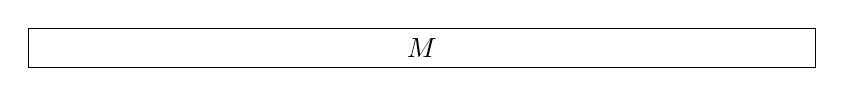
\begin{tikzpicture}[scale=0.5]
  \draw (0,0) rectangle (20,1);
  \node at (10, 0.5) {$M$};
\end{tikzpicture}
\end{center}

\subsubsection{Signed values, $\mathbb Z$}

Two pieces of information need to be represented: the sign and the absolute value (or magnitude). 

Explicit sign:
\begin{center}
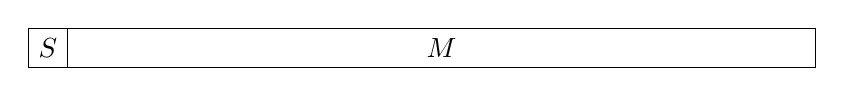
\begin{tikzpicture}[scale=0.5]
  \draw (0,0) rectangle (1,1);
  \draw (1,0) rectangle (20,1);
  \node at (0.5, 0.5) {$S$};
  \node at (10.5, 0.5)  {$M$};
\end{tikzpicture}
\end{center}

Implicit sign:
\begin{center}
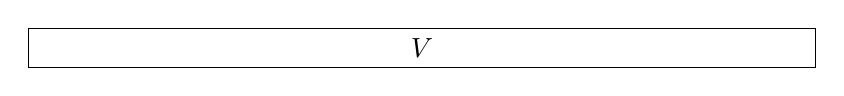
\begin{tikzpicture}[scale=0.5]
  \draw (0,0) rectangle (20,1);
  \node at (10, 0.5) {$V$};
\end{tikzpicture}
\end{center}

Representation usually have an explicit sign:
\begin{itemize}
\item Sign-and-magnitude,
\item One's complement,
\item Two's complement,
\item Excess-K,
\end{itemize}
but can also have an implicit sign like Base-2.

Two's complement is the most used.

\textbf{Sign-and-magnitude}

This representation is the intuitive way of expressing signedness.

\begin{tabular}{cc}
S & M \\
1 & N-1
\end{tabular}

Range is $[-127, +127]$.
Zero is encoded as $-0$ and $+0$:
\begin{equation*}
\begin{bmatrix}0\;0\;0\;0\;0\;0\;0\;0 \end{bmatrix}
\end{equation*}
\begin{equation*}
\begin{bmatrix}1\;0\;0\;0\;0\;0\;0\;0 \end{bmatrix}
\end{equation*}

The definition of two zero and the impossibility of representing the subtraction in an efficient way are strong limitations.

\textbf{One's complement}

Negative values consists of applying a bitwise NOT operator to the unsigned representation.

Range is $[-127, +127]$.
Zero is encoded as $-0$ and $+0$:
\begin{equation*}
\begin{bmatrix}0\;0\;0\;0\;0\;0\;0\;0 \end{bmatrix}
\end{equation*}

\begin{equation*}
\begin{bmatrix}1\;1\;1\;1\;1\;1\;1\;1 \end{bmatrix}
\end{equation*}

Hard to implement in pratice: \textit{end-around carry}: if $1$ is carried then it is added back. This representation has been abandoned.

\textbf{Two's complement}

Most used representation developed to workaround the double zero and the carry issue: if $1$ is carried is is simply ignored.

Negative values consists of applying a bitwise \texttt{NOT} operator to the unsigned representation and adding $1$.

Range is $[-128, +127]$:  notice that it is not symmetric anymore.

Zero is encoded uniquely as:
\begin{equation*}
\begin{bmatrix}0\;0\;0\;0\;0\;0\;0\;0 \end{bmatrix}
\end{equation*}

Representation of the bounds:

\begin{equation*}
+127:\qquad\begin{bmatrix}0\;1\;1\;1\;1\;1\;1\;1 \end{bmatrix}
\end{equation*}
\begin{equation*}
-127:\qquad\begin{bmatrix}1\;0\;0\;0\;0\;0\;0\;1 \end{bmatrix}
\end{equation*}
\begin{equation*}
-128:\qquad\begin{bmatrix}1\;0\;0\;0\;0\;0\;0\;0 \end{bmatrix}
\end{equation*}

Motivation: the subtraction can be implemented like an addition since:
\begin{equation*}
[+x]_2\;+\;[-x]_2 = [0]_2
\end{equation*}

Take the simple example of: $+ 127 - 127$
\begin{equation*}
\begin{split}
+127\qquad\begin{bmatrix}0\;1\;1\;1\;1\;1\;1\;1 \end{bmatrix}\\
-127\qquad\begin{bmatrix}1\;0\;0\;0\;0\;0\;0\;1 \end{bmatrix}\\
\ = 0 \qquad 1 \begin{bmatrix}0\;0\;0\;0\;0\;0\;0\;0 \end{bmatrix}
\end{split}
\end{equation*}

\subsection{Real numbers}

The difficulty to represent infinitely many real numbers with a finite number of bits: only some numbers can be represented exactly.
A number is binary rational if it can be written exactly in base $2$.

Other number are then approximated: the error due to the representation is coined \textit{round-off error}.

\begin{equation*}
\begin{bmatrix}527.2\end{bmatrix}_{10} = 1\cdot 2^{+9} + 1\cdot 2^{+3} + 1\cdot 2^{+2} + 1\cdot 2^{1} + 1\cdot 2^{0} + 0\cdot 2^{-1} + 0\cdot 2^{-2} + 1\cdot 2^{-3}+ 1\cdot 2^{-4} + \cdots
\end{equation*}
\begin{equation*}
\begin{bmatrix}527.2\end{bmatrix}_{10} \approx \bigl(+1\bigr)\cdot 2^{+9}\;\bigl(1\cdot 2^{+0} + 1\cdot 2^{-6} + 1\cdot 2^{-7} + 1\cdot 2^{-8} + \cdot 2^{-9} + 0\cdot 2^{-10} + 1\cdot 2^{-11}+ 1\cdot 2^{-12}\bigr)
\end{equation*}

\begin{equation*}
\begin{bmatrix}527.2\end{bmatrix}_{10} \approx \bigl(+1\bigr)\cdot 2^{+9}\;\begin{bmatrix}1.0000011110011\end{bmatrix}_{2}
\end{equation*}

\begin{equation*}
\bigl(+1\bigr)\cdot 2^{+9}\;\begin{bmatrix}1.0000011110011\end{bmatrix}_{2} = 527.1875
\end{equation*}

%(8435)10

IEEE754: standard defining the properties of floating-point operations.

Definition of:
\begin{itemize}
\item guard digits to reduce the error when subtracting two nearby digits,
\item algorithms for:
\begin{enumerate}
\item addition
\item subtraction
\item multiplication
\item division
\item square root
\end{enumerate}
\end{itemize}

\subsubsection{Fixed-point values}

\begin{center}
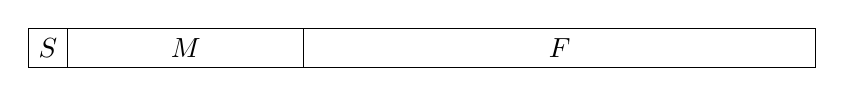
\begin{tikzpicture}[scale=0.5]
  \draw (0,0) rectangle (1,1);
  \draw (1,0) rectangle (7,1);
  \draw (7,0) rectangle (20,1);
  \node at (0.5, 0.5) {$S$};
  \node at (4, 0.5) {$M$};
  \node at (13.5, 0.5) {$F$};
\end{tikzpicture}
\end{center}

\subsubsection{Floating-point values}

\begin{center}
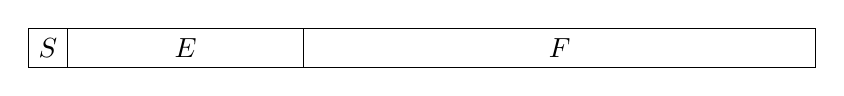
\begin{tikzpicture}[scale=0.5]
  \draw (0,0) rectangle (1,1);
  \draw (1,0) rectangle (7,1);
  \draw (7,0) rectangle (20,1);
  \node at (0.5, 0.5) {$S$};
  \node at (4, 0.5) {$E$};
  \node at (13.5, 0.5) {$F$};
\end{tikzpicture}
\end{center}



\subsubsection{Denormalization}

Smallest numbers that can be represented using the first bit.

Minimum: $2^{1-b-f}$

Single precision: $2^{-149}\;\approx 1.6\cdot 10^{-45}$
Double precision: $2^{-1074}\;\approx 5.0\cdot 10^{-324}$

\subsection{Data model}

\begin{center}
\input{\data/data-models}
\end{center}



\subsection{Von Neumann model}


\subsubsection{Description}

Description

\subsubsection{Improvements}

Caching: higher speed of smaller memory, keep some data in a fast memory if it is reused.

\subsubsection{Memory hierarchy}

Locality is crucial to achieve performance, it is based on heuristics.

Temporal locality: how likely will we need the data in the future?

Spatial locality: how likely will we need the data in the block of memory?

Memory stall cycles: number of cycles during which the processor is stalled, waiting for a memory access.

\section{Implementation of a processor}

In this part a processor is a conceptual unit able to load data, perform computations and store the result.


\section{Different types of parallelism}

\subsection{Pipelining}

Multiple instructions are overlapped in execution: take advantage of parallelism existing between actions required to execute an instruction.

View of an assembly line:

Prototypical Five-Stage RISC:
\begin{tabular}{c|l|l|}
\textbf{IF}  & Instruction-Fetch  & \\
\textbf{ID}  & Instruction-Decode & \\
\textbf{EX}  & Execute            & \\
\textbf{MEM} & Memory Access      & Load/Store \\
\textbf{WR}  & Write in Register  & Register-Register, ALU, Load\\
\end{tabular}

The theoretical speed-up for a $N$--stage is $N$, but:
\begin{itemize}
\item Overhead for controlling the pipeline.
\item Lowest common denominator: speed is limited to the slowest element.
\item Hazards.
\end{itemize}

The last element \textit{Hazards} comprises:
\begin{itemize}
\item 
\end{itemize}

Rule:
\begin{itemize}
\item Deeper pipe: increased throughput, but increased penalty.
\end{itemize}

\subsection{Superscalar execution}

\subsection{Vectorization}

\subsection{Caching}

Problem: the memory latency has increased relative to the CPU frequency, moving data from/to the memory is expensive relative to computational cost on the CPU.


\begin{enumerate}
\item Cache hit: the processor find the data in the cache
\item Cache miss: the processor does not find the data in the cache
\end{enumerate}

Cache miss penalty depends on:
\begin{enumerate}
\item the memory latency: time to access the first block.
\item the memory bandwidth: time of transfer per unit block.
\end{enumerate}

Using locality to buffer reuse of reoccurring items.

\medskip
Different cache strategies based on different implementations of:
\begin{enumerate}
\item block placement: where is the cached data stored?
\item block identification: how is the data found in the cache?
\item block replacement: how to decide which block should be replaced?
\item write strategy: if data is changed, how to write to the main memory?
\end{enumerate}

\subsubsection{Placement}
\begin{itemize}
\item \textit{direct-mapped}: block can be placed only at one location
\item \textit{fully associative}: block can be placed anywhere
\item \textit{set associative}: block can be placed in a restricted set of places, ``n-way associative'' means that nw
\end{itemize}

\subsubsection{Identification}

The block is assigned an address tag to 

\subsubsection{Replacement}

\begin{itemize}
\item \textit{Random}: block replaced is chosen randomly
\item \textit{FIFO}: First-In-First-Out
\item \textit{LRU}: Least-Recently-Used
\item \textit{pseudo-LRU}: Least-Recently-Used with heuristics
\end{itemize}

\subsubsection{Write strategy}

\begin{itemize}
\item \textit{Write-though}: write to main memory directly
\item \textit{Write-back}: write a next synchronization
\end{itemize}

\subsection{Speculative and Out-of-Order execution}

During the execution there may exist dependencies between data such that the process needs to wait for data before proceeding further.

\begin{enumerate}
\item \textit{in-order}: pause of execution until data is fetched
\item \textit{out-of-order}: instruction waits but execution of other instructions with non-dependent data is scheduled.
\end{enumerate}


\end{document}
